\documentclass[12pt]{article}
\title{3D Software Rasterisation Renderer \\ \large Com S 424 Final Project}
\author{Ian Malerich \\ imm@iastate.edu}
\usepackage{amssymb, amsfonts, amsthm, mathtools, graphicx, breqn}
\usepackage{minted, subfig, float, scrextend, setspace, soul, caption, subcaption}
\usemintedstyle{friendly}
\usepackage[hidelinks]{hyperref}

\onehalfspacing
\begin{document}
\raggedright

\maketitle

\section*{Introduction}

This project implements a rendering system for 3 dimensional graphics, defined as a set
of triangles in 3 dimensional space. Models are input via a .obj file containing triangle data
as well as a .mtl referenced by the .obj file which holds texture information. A camera is set
at the origin looking down the z-axis and captures a single image representing the scene.
Therefore the problem size varies across two primary variables: the number of triangles which
need to be rendered and the dimensions of the output texture, that is, how many pixel need
to be colored.

\bigbreak
\begin{center}
	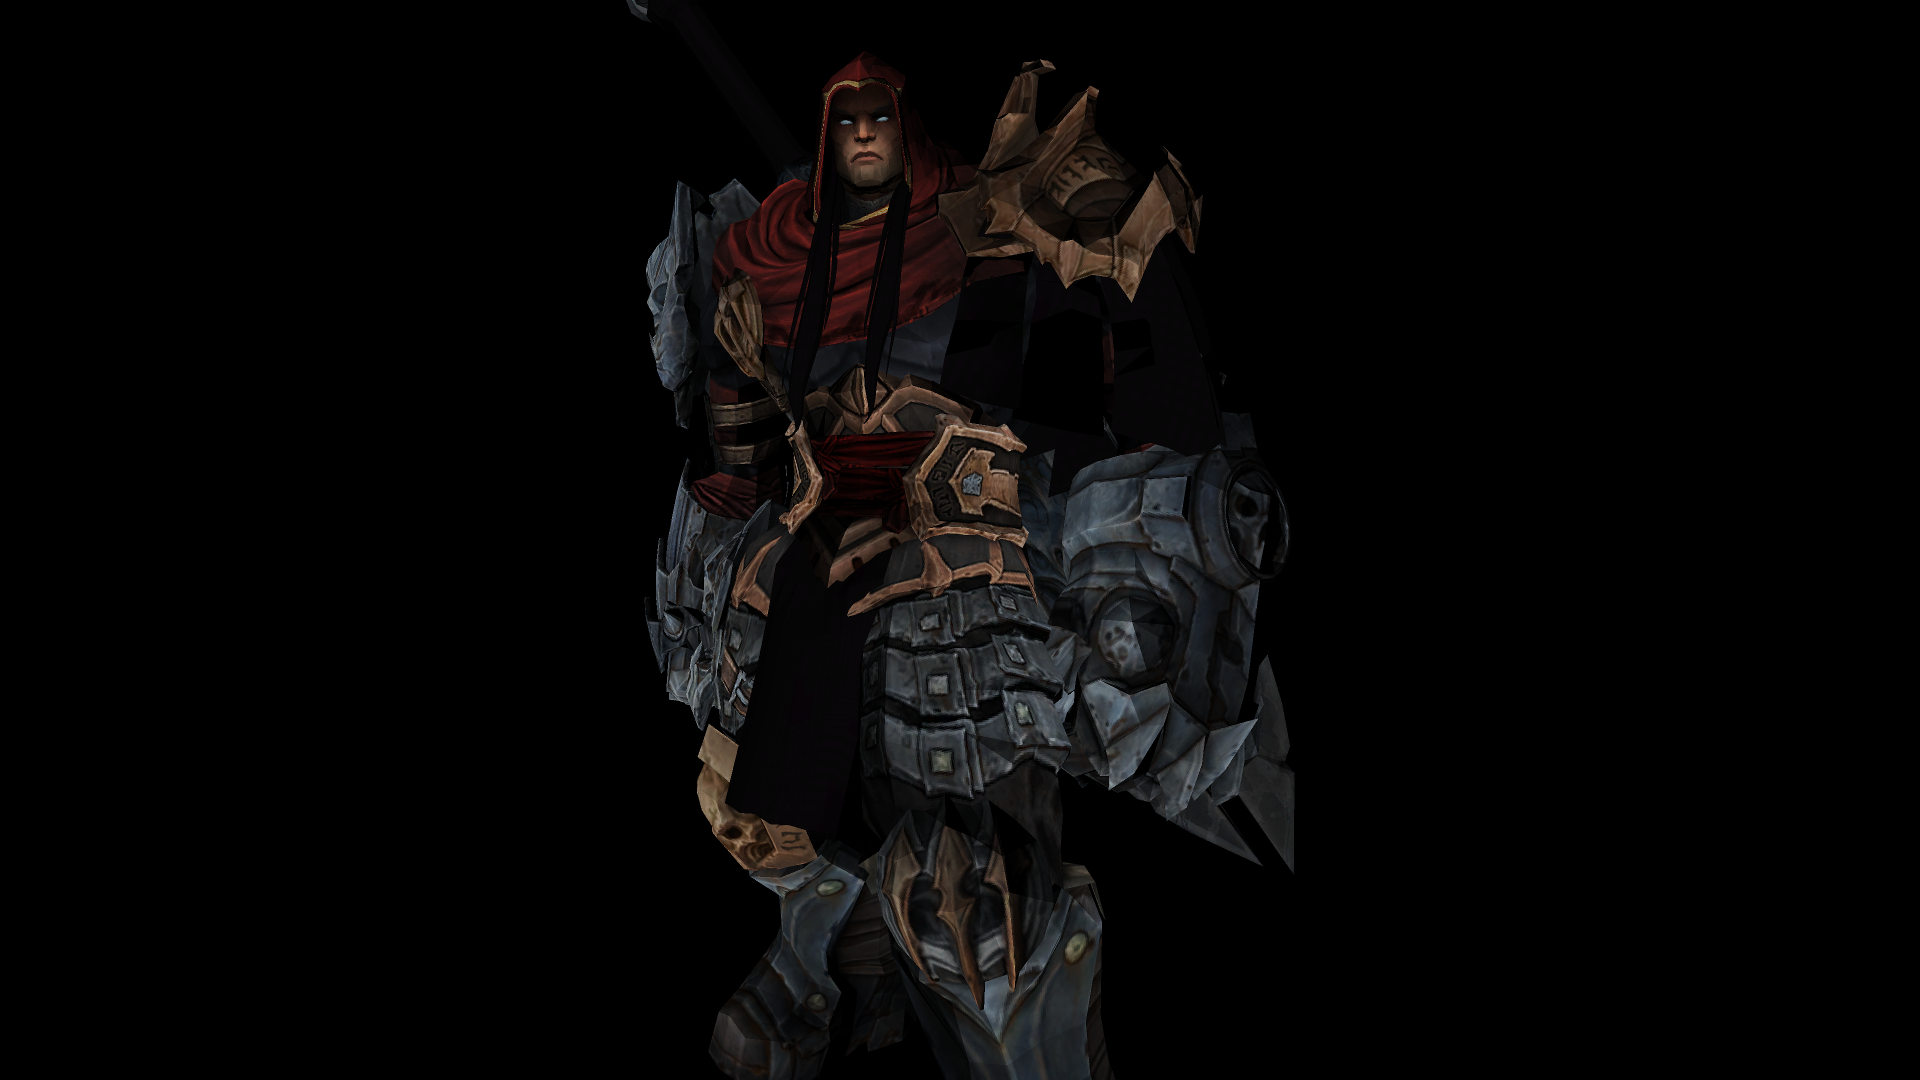
\includegraphics[scale=0.13]{war.png}
\end{center}

\clearpage
\section*{Systems}

Results are included for both my personal system and the hpc cluster. The below chart provides some basic
information about each system as read from /proc/cpuinfo.

\bigbreak
\begin{center}
	\begin{tabular}{|l|c|c|}
		\hline
		system & personal & hpc-class \\ \hline \hline
		model name & i7-3630QM & Xeon CPU-E5-2650 \\ \hline
		cores & 4 & 8 \\ \hline
		nproc & 8 & 13 \\ \hline
		clock speed & 2.40GHz & 2.00GHz \\ \hline
		cache size & 6144 KB & 20480 KB \\ \hline
		address size (physical) & 36 bits & 46 bits \\ \hline
		address size (virtual) & 48 bits & 48 bits \\ \hline
	\end{tabular}
\end{center}

\section*{Models}

Below are a list of models which will be used for various performance tests as well as how many
vertices make up the model. Note that each model has accompanying textures which will affect memory
usage but in terms of performance texture samples are handled per pixel and thus the output image
size is the bigger concern and not buffer size.
It is worth mentioning that while the model 'war' has the least vertices, it is the only model
not made up of a single mesh. Rather, war is made up by 10 smaller models each with their own texture.
Thus as the provided graphs will demonstrate the performance of this mesh does not quite fall in line
with the other models.

\begin{center}
	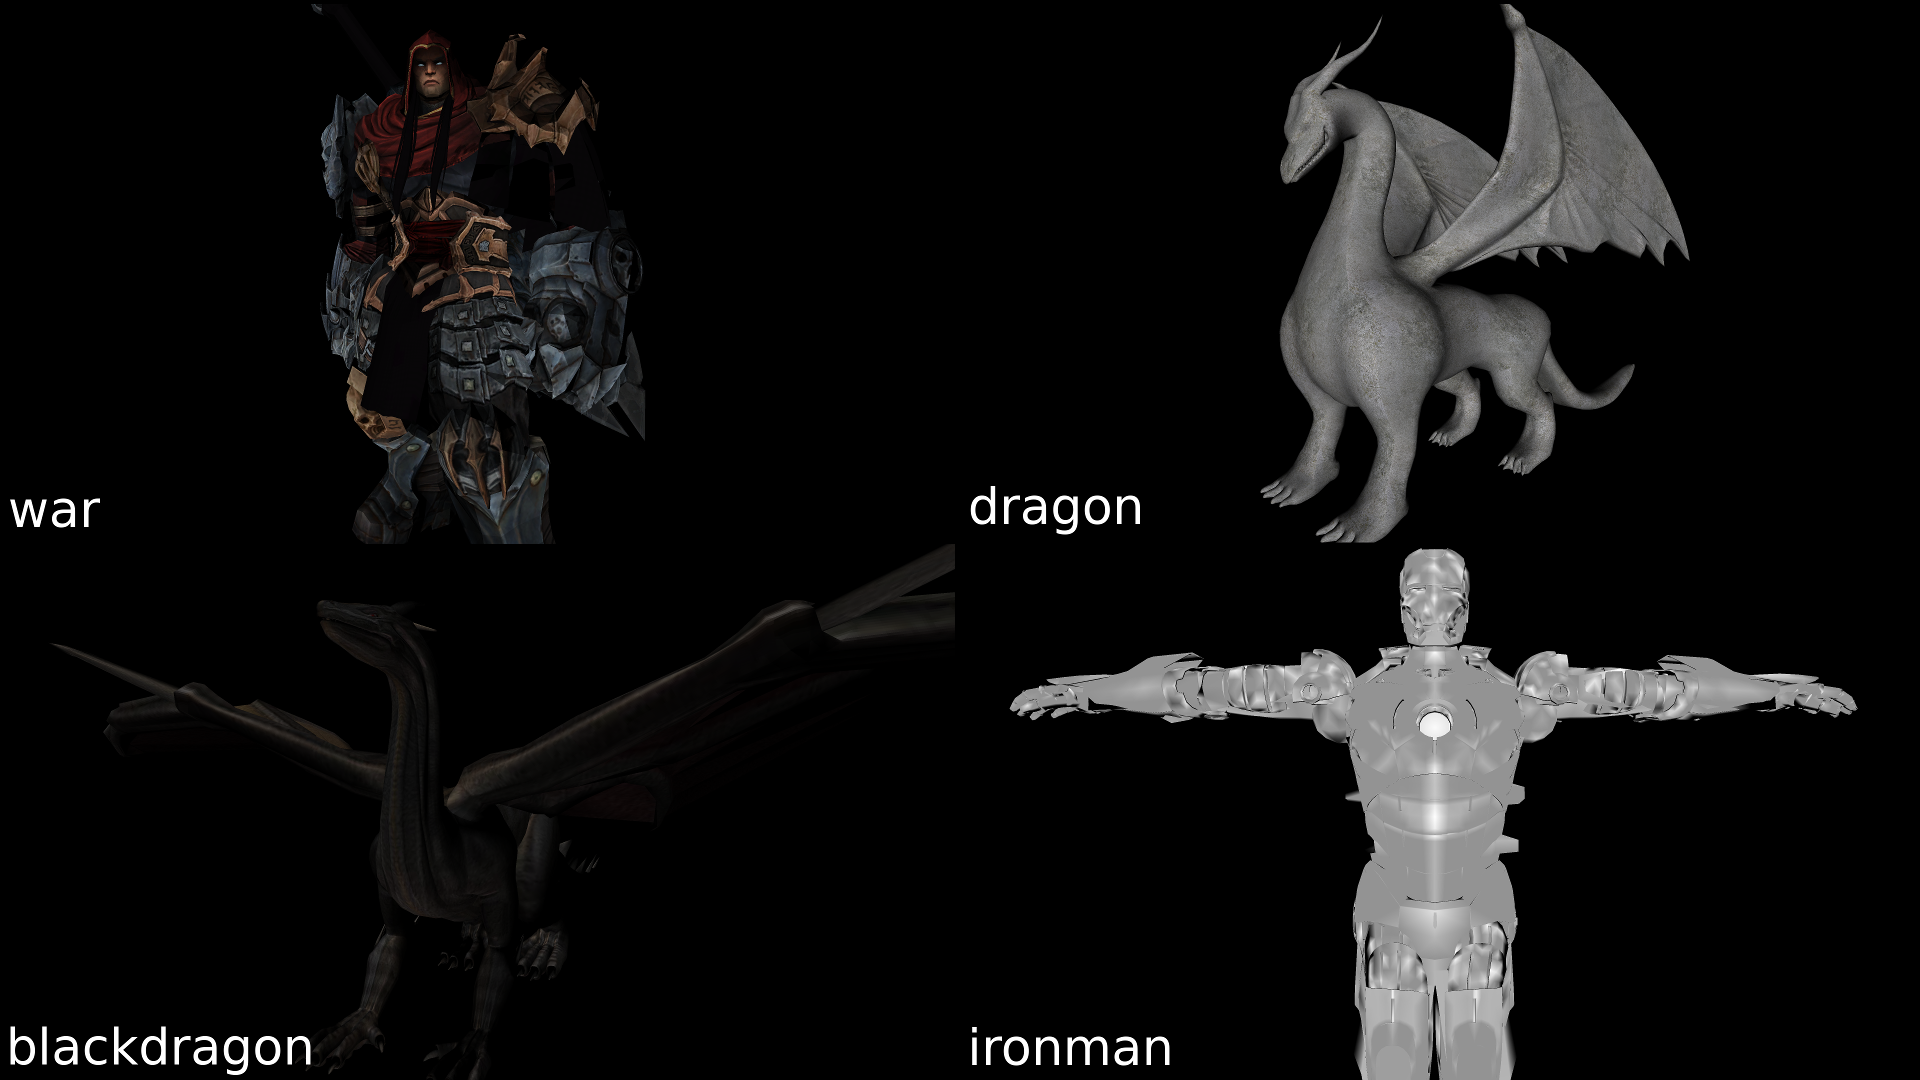
\includegraphics[scale=0.225]{models.png}
\end{center}

\bigbreak
\begin{center}
	\begin{tabular}{|l|c|c|}
		\hline
		name & vertex count & parts \\ \hline \hline
		war & 44,115 & 10 \\ \hline
		dragon & 61,152 & 1 \\ \hline
		blackdragon & 113,955 & 1 \\ \hline
		iron man & 596,682 & 1 \\ \hline
	\end{tabular}
\end{center}

\section*{Measurements}

The primary goal in regards to performance is to minimize total rendering time. To that respect, I will
not be including model and texture load times as well as output image write time in any measurements. 
The clock will begin at the start at the rendering process and end once rendering is complete.

\section*{Serial Execution}

Below we can see how well my code performs when running in serial. We can clearly see that the output
image resolution has a much greater influence on total render time. Number of vertices does tend to
produce longer render times but the increase is much more gradual. Note that an output image of 
size $3840\times2160$ (orange) is exactly $4\times$ that of $1920\times1080$ (blue) thus based only on results so far
render time appears to scale almost linearly with image resolution. Regardless, based on this graph
our concern is much less with vertex transformations and much more with pixel rendering.

\begin{center}
	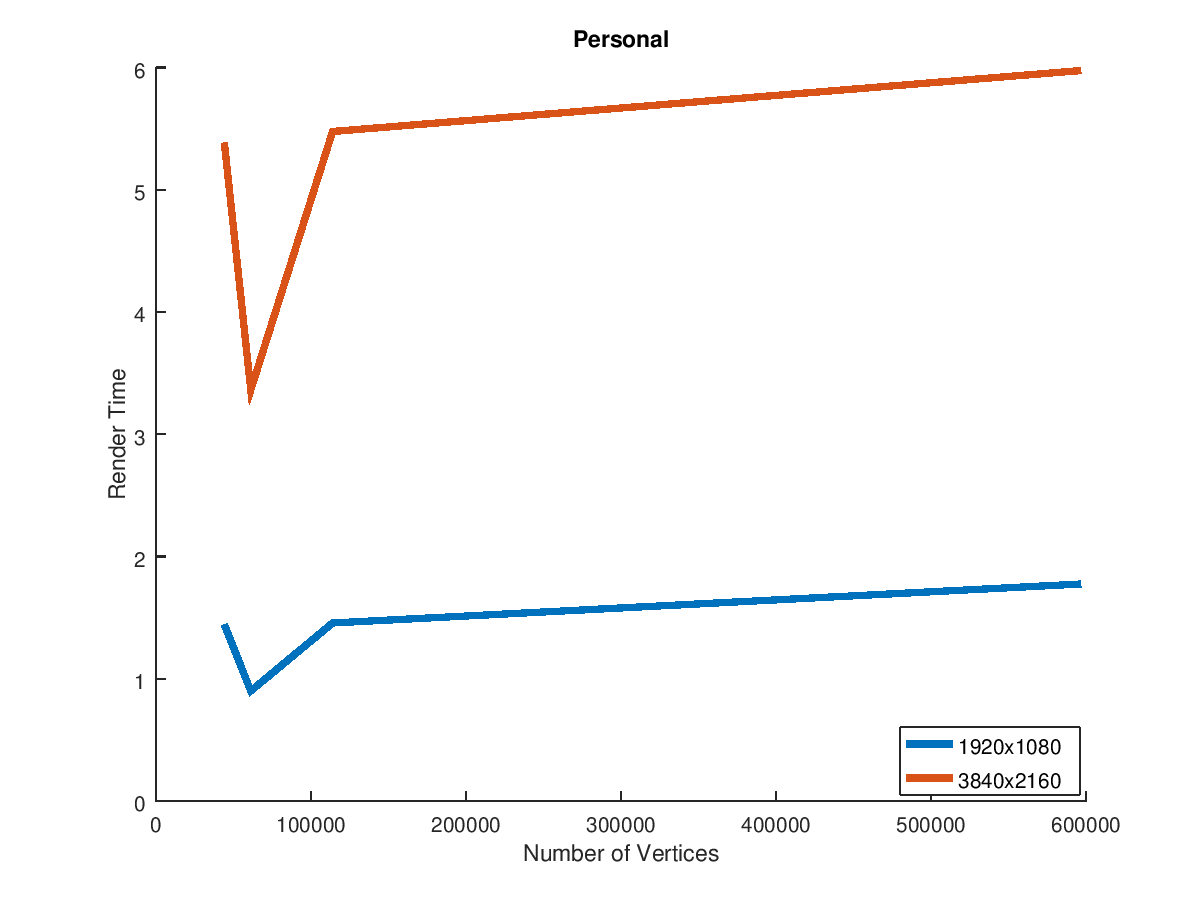
\includegraphics[scale=0.5]{serial_personal.png}
\end{center}

I ran the valgrind profiler `callgrind' on the blackdragon mesh at a resolution of $3840\times2160$ to see
exactly how much time was spent in code. The table below contains relevant data produced by callgrind.
Note I have ommitted calls involved in model/texture loading which require compressions/disk access beyond
my control and concern.

\begin{center}
	\begin{tabular}{|r|l|l|}
		\hline
		Ir & Function & Primary Use \\ \hline
		2,927,228,239 & isPointInTriangle & Should a pixel be drawn for a give triangle. \\ \hline
		2,793,061,201 & vecCross & Find bary centric coords for vertex interpolation. \\ \hline
		1,739,333,716 & drawTriangle & Interplate data and fill pixels. \\ \hline
		1,239,622,129 & sampleNearest & Sample a color from a texture. \\ \hline
		647,909,164 & sampleLinear & Interpolate 4 nearest samples from a texture.\\ \hline
		509,067,930 & roundf & Round coordinates for texture sampling. \\ \hline
		426,630,011 & simpleShader() & Color in a given pixel. \\ \hline
	\end{tabular}
\end{center}

All top calls which influence the measurements I am taking directly relate pixel rendering and not
vertex transformations. Confirming what we noted about the serial execution graph. This tells us 
that while improved vertex transformations may help our performance, the bigger gains are to be made
from parallelizing the pixel rendering code.

\section*{Parallelization}

The easiest method, and the first method I will try, to parallelize this code is a simple parallel for
directive loop over each face. Each thread will then transform 3 vertices corresponding to its assigned
face, and then draw the given triangle. Within the draw\_triangle method critical sections are needed
when writing to the back and output buffers so that only one thread may write at a time. All other
operations may be performed in parallel.

\begin{minted}[linenos, tabsize=2]{c}
#pragma omp parallel for num_threads(thread_count)
for (int i=0; i<num_faces(m); i++) {
	transform_vertex(&m.vertices[3*i + 0], &proj, WIDTH, HEIGHT);
	transform_vertex(&m.vertices[3*i + 1], &proj, WIDTH, HEIGHT);
	transform_vertex(&m.vertices[3*i + 2], &proj, WIDTH, HEIGHT);

	draw_triangle(&m, i, simple_shader, m.material, buffer, 
		back_buffer, SIZE);
}
\end{minted}
\bigbreak
\begin{minted}[linenos, tabsize=2]{c}
#pragma omp critical
{
	if (back[y*buffer_size.x + x] > pos.z) {
		back[y*buffer_size.x + x] = pos.z;

		// interpolate vertex data
		vector_t tex_coord = interpolate(tex_coords, 
			bc_screen);
		vector_t norm = interpolate(norms, bc_screen);
		vector_t tan = interpolate(tans, bc_screen);

		vector_t c = shader((shader_data_t){pos, 
			tex_coord, norm, tan}, material);
		draw_point(vector_to_point(pos), 
			vector_to_color(c), buffer, buffer_size);
	}
}
\end{minted}

The immediate issue with this is the giant critical section surrounding the pixel
rendering code. We found by analyzing the serial implementation that this is where the 
majority of our work will take place and by forcing it into a critical section we are
severely limiting the potential performance gains. Nevertheless, we still see a performance
increase when introducing threading, although limited to just a few threads. Additional threads
likely do not provide enough added benefit to overcome the limitations of the per pixel critical section.

\begin{center}
	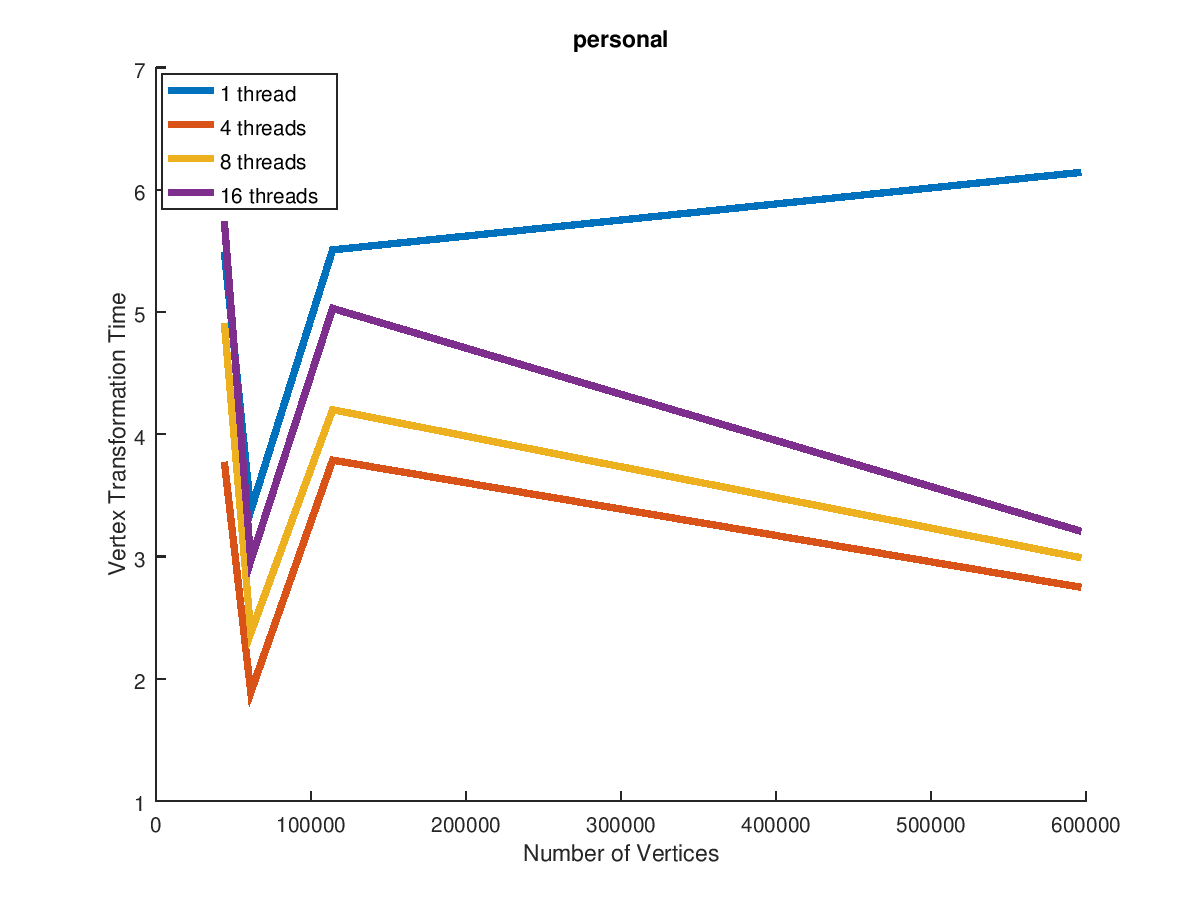
\includegraphics[scale=0.5]{parallel0_personal.png}
\end{center}
\textcolor[RGB]{200,200,200}{\rule{\textwidth}{0.75pt}}\bigbreak

Note that vertex transformation code is entirely independent each triangle. As such, we can split
our vertex transformation code and triangle rasterization code into separate loops. 
This exemplifies the idea that these are the two dimensions on which the program scales. By doing
this if a thread would be stuck waiting for a critical section in the old code, it can now continue
to transform vertices in parallel. By using this method, we can see a very slight but insignificant
increase in performance, particularly when number of threads is large.

\begin{minted}[linenos, tabsize=2]{c}
#pragma omp parallel for num_threads(thread_count)
for (int i=0; i<m.vert_count; i++) {
	transform_vertex(&m.vertices[i], &proj, WIDTH, HEIGHT);
}

#pragma omp parallel for num_threads(thread_count)
for (int i=0; i<num_faces(m); i++) {
	draw_triangle(&m, i, simple_shader, m.material, buffer, 
		back_buffer, SIZE);
}
\end{minted}

\begin{center}
	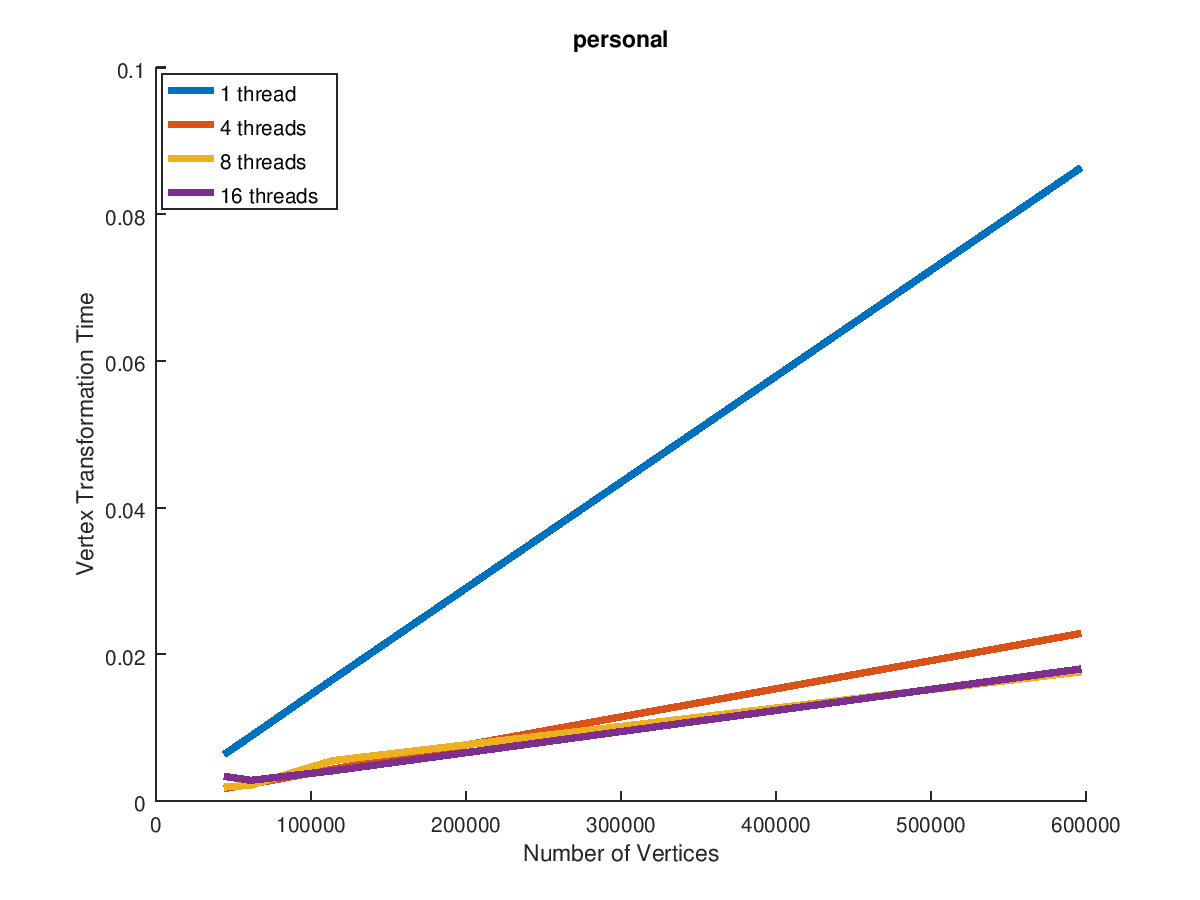
\includegraphics[scale=0.5]{parallel1_personal.png}
\end{center}
\textcolor[RGB]{200,200,200}{\rule{\textwidth}{0.75pt}}\bigbreak

To get over the critical section hurdle, we could introduce a lock 
for each given pixel. We can have multiple threads writing to buffers
so long as they are not writing to the same location (triangles can overlap!).
However locks can be slow and for a $3840\times2160$ image we would require 8.3 million
locks, which would need a lock and unlock for every single write. This seems highly
impractical and not likely to solve anything. Thus I will ignore this strategy.
\bigbreak
A much better approach would be to run the rasterization step in parallel. That is,
we loop through triangles on our main thread, and then spawn a set of threads which 
iterate over the bounding region of that triangle. Thus each per pixel operation can be
performed in parallel. Further since each pixel within a bounding box is unique, we can 
guarantee each thread is reading/writing to a unique location in the back and output buffers.
Thus no critical section is necessary in the below implementation.

\begin{minted}[linenos, tabsize=2]{c}
#pragma omp parallel for num_threads(thread_count)
for (int i=0; i<m.vert_count; i++) {
	transform_vertex(&m.vertices[i], &proj, WIDTH, HEIGHT);
}

for (int i=0; i<num_faces(m); i++) {
	draw_triangle(&m, i, simple_shader, m.material, buffer, 
		back_buffer, SIZE);
}
\end{minted}
\bigbreak
\begin{minted}[linenos, tabsize=2]{c}
#pragma omp parallel for num_threads(thread_count)
for (int idx = 0; idx < count; idx++) {
	int x = (idx % width) + bbox.min.x;
	int y = (idx / width) + bbox.min.y;

	vector_t pos = make_vector(x, y, 0, 0);

	if (is_point_in_triangle(pos, vertices)) {
		// compute bary centric coordinates, 
		// we will need this for our depth test
		vector_t bc_screen = 
			bary_centric(make_vector(x,y, 0.0, 0.0), vertices);
		if (bc_screen.x < 0 || bc_screen.y < 0 || bc_screen.z < 0) 
			{ continue; }
		pos.z = (vertices[0].z * bc_screen.x) + 
			(vertices[1].z * bc_screen.y) + 
			(vertices[2].z * bc_screen.z);

		if (back[y*buffer_size.x + x] > pos.z) {
			back[y*buffer_size.x + x] = pos.z;

			// interpolate vertex data
			vector_t tex_coord = 
				interpolate(tex_coords, bc_screen);
			vector_t norm = interpolate(norms, bc_screen);
			vector_t tan = interpolate(tans, bc_screen);

			vector_t c = shader((shader_data_t){pos, tex_coord, 
				norm, tan}, material);
			draw_point(vector_to_point(pos), vector_to_color(c), 
				buffer, buffer_size);
		}
	}
}
\end{minted}

In the graph below we can see much larger increases in performance than we have 
experienced before. Even the most complex models can be rendered in just over 2 seconds
with the simplest approaching 1 second. Note that on my personal system a huge spike upwards 
occurs for $>8$ threads, this is not particularly of interest as my system cannot run any more than
8 threads at a given time thus using more only incurs additional overhead.

\begin{center}
	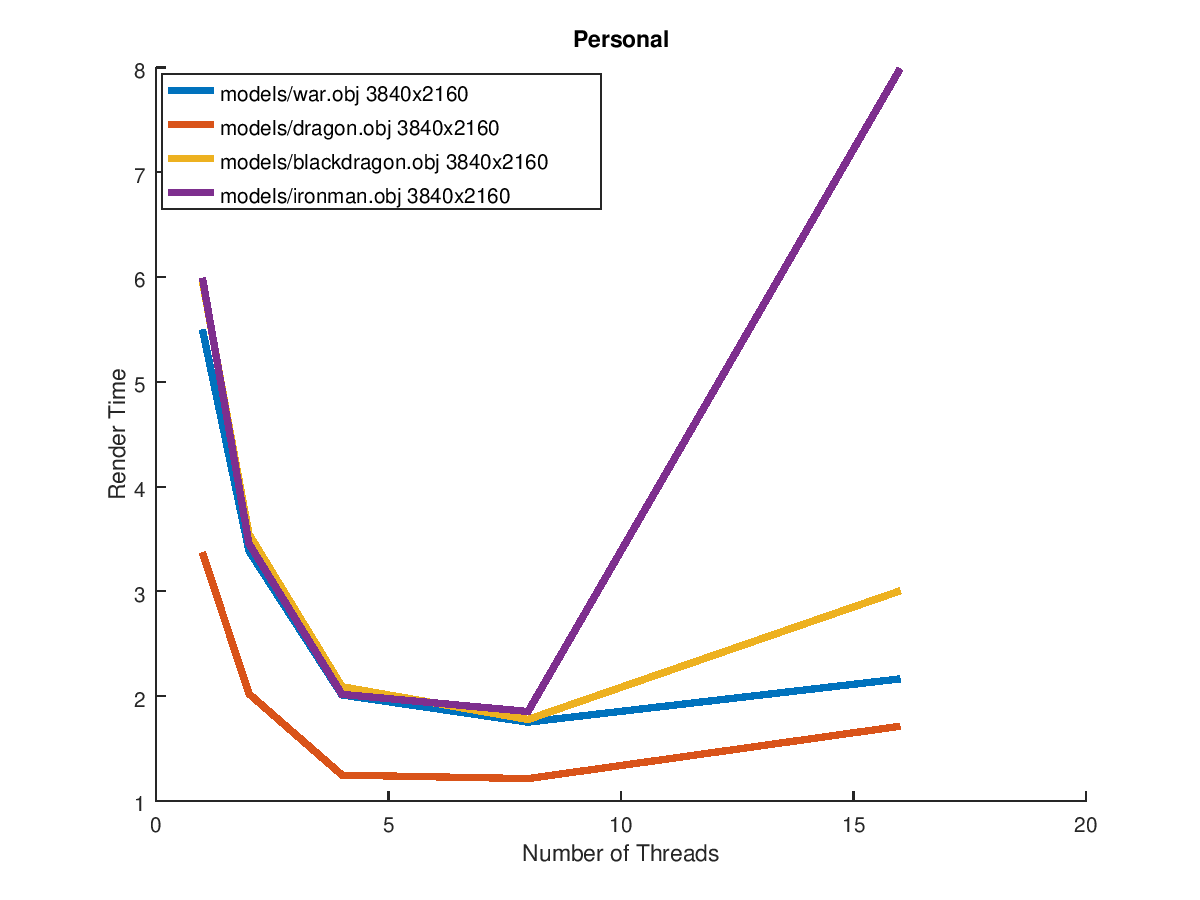
\includegraphics[scale=0.5]{parallel2_personal.png}
\end{center}

\section*{Method Comparison}

In all cases, ironman took the most significant amount of time to render. The graph below
shows a comparison between the 3 methods in rendering this model at $3840\times2160$. We can see
the final solution branching off from the other methods starting particularly at $4+$ threads.
Interestingly, we can see Method 3 is hit the hardest when run on too many threads, though clearly
in all other cases it performs the best.

\begin{center}
	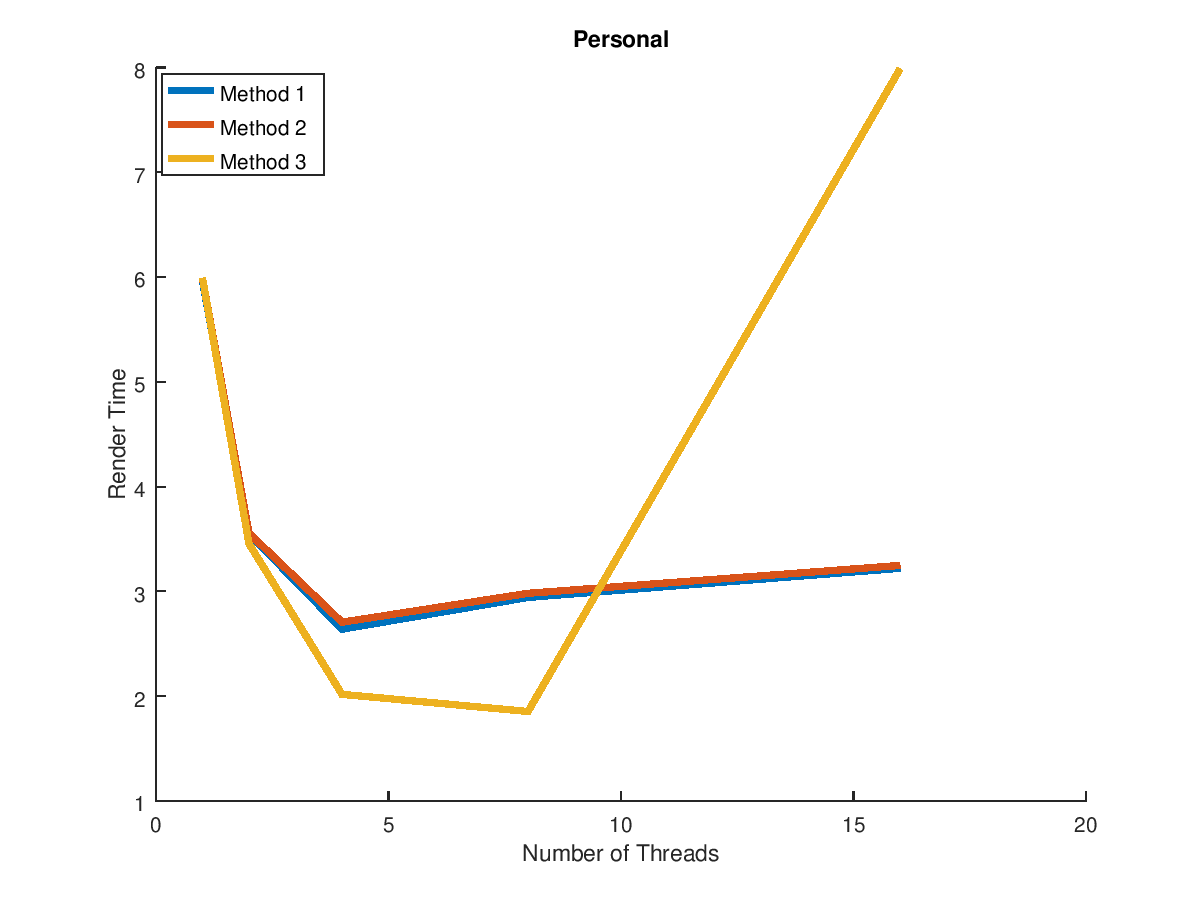
\includegraphics[scale=0.5]{parallel3_personal.png}
\end{center}

\section*{OpenMP Scheduling}

Using Method 3, the following graphs analyze different OpenMP scheduling methods and chunk sizes.
With the exception of (dynamic, 1) performing notably terrible, they all seem relatively close in performance
to each other and all follow the same overall trends. It appears larger chunk sizes provide the best performance.
This is likely due to the fact that each operation is relatively short and thus threads will benefit having
nearby memory for their next computation, a trait that a larger chunk size provides.
\begin{center}
	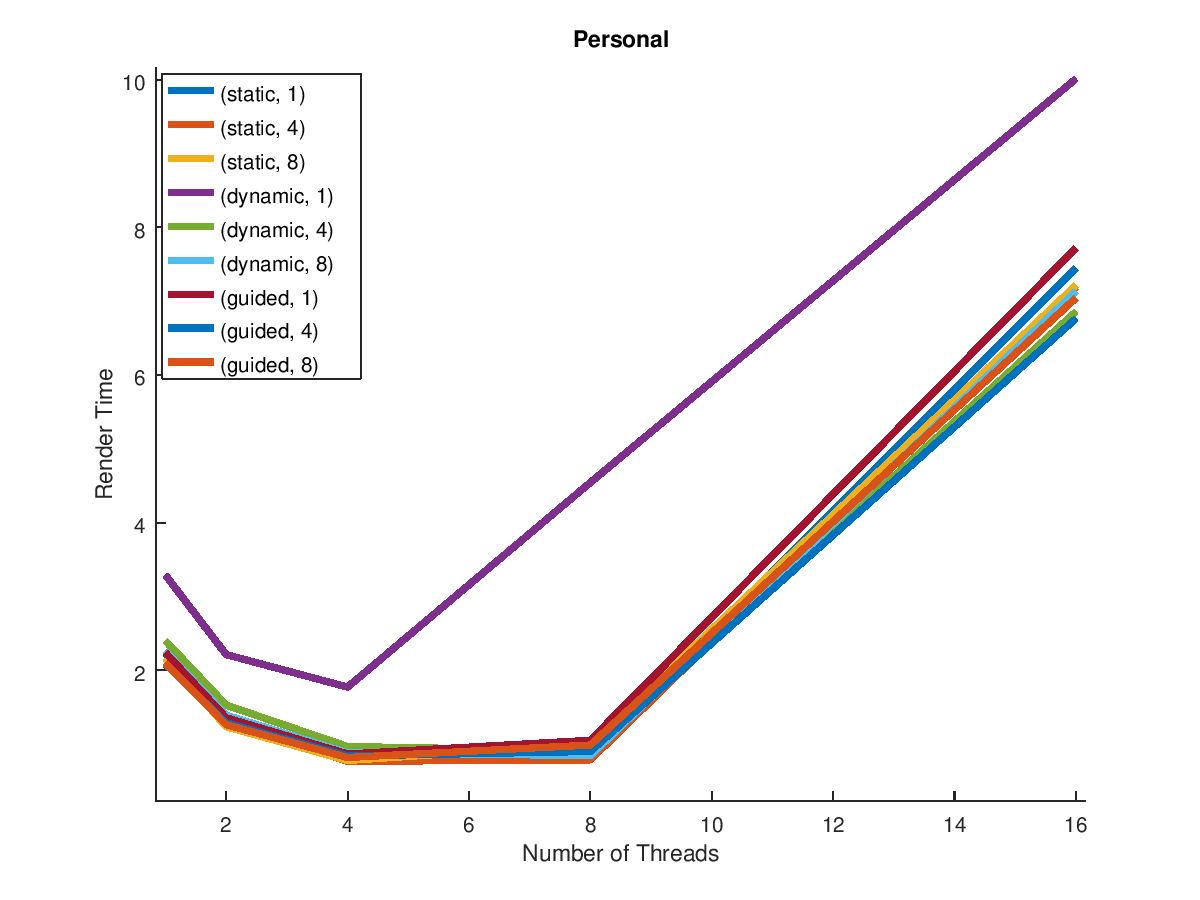
\includegraphics[scale=0.5]{scheduling_personal.png}
\end{center}
Running static distrubition with various chunk sizes shows that the chunk size can clearly be too large.
Sizes 64 and 128 are particularly terrible. Chunk sizes between 4 and 32 seem to perform the best.
\begin{center}
	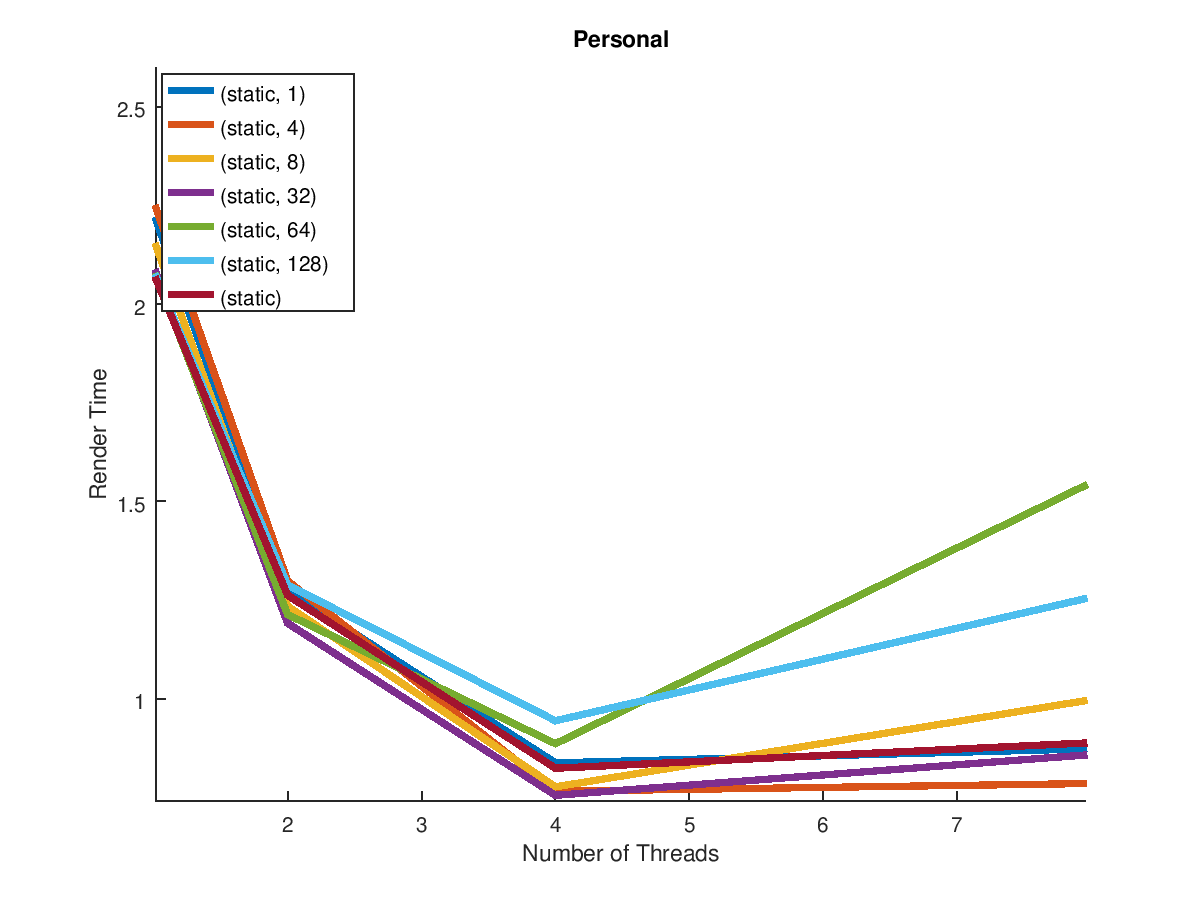
\includegraphics[scale=0.5]{static_personal.png}
\end{center}

\section*{Conclusion}

\clearpage
\section*{References}

\begin{itemize}
	\item Lengyel, Eric. \textit{Mathematics for 3D Game Programming and Computer Graphics.} Course Technology,
Cengage Learning, 2012.
	\item Sokolov, Dmitry. ``Tinyrenderer". \url{https://github.com/ssloy/tinyrenderer/wiki}
	\item Barrett, Sean. ``stb". \url{https://github.com/nothings/stb}
	\item Michael S\"uB and Claudia Leopold. \textit{Common Mistakes in OpenMP and How To Avoid Them}.
\end{itemize}

\end{document}
